\documentclass{standalone}
\usepackage[dvipsnames]{xcolor}

\usepackage{tikz}
\usetikzlibrary{arrows.meta,shapes.geometric,positioning,matrix,calc,fit,decorations.pathreplacing}

\colorlet{States}{Melon!50}
\colorlet{Energies}{SkyBlue!50}
\colorlet{Rect}{Orchid!30}
\colorlet{Decision}{GreenYellow!30}
\colorlet{Frame1}{Magenta}
\colorlet{Frame2}{NavyBlue}


\begin{document}

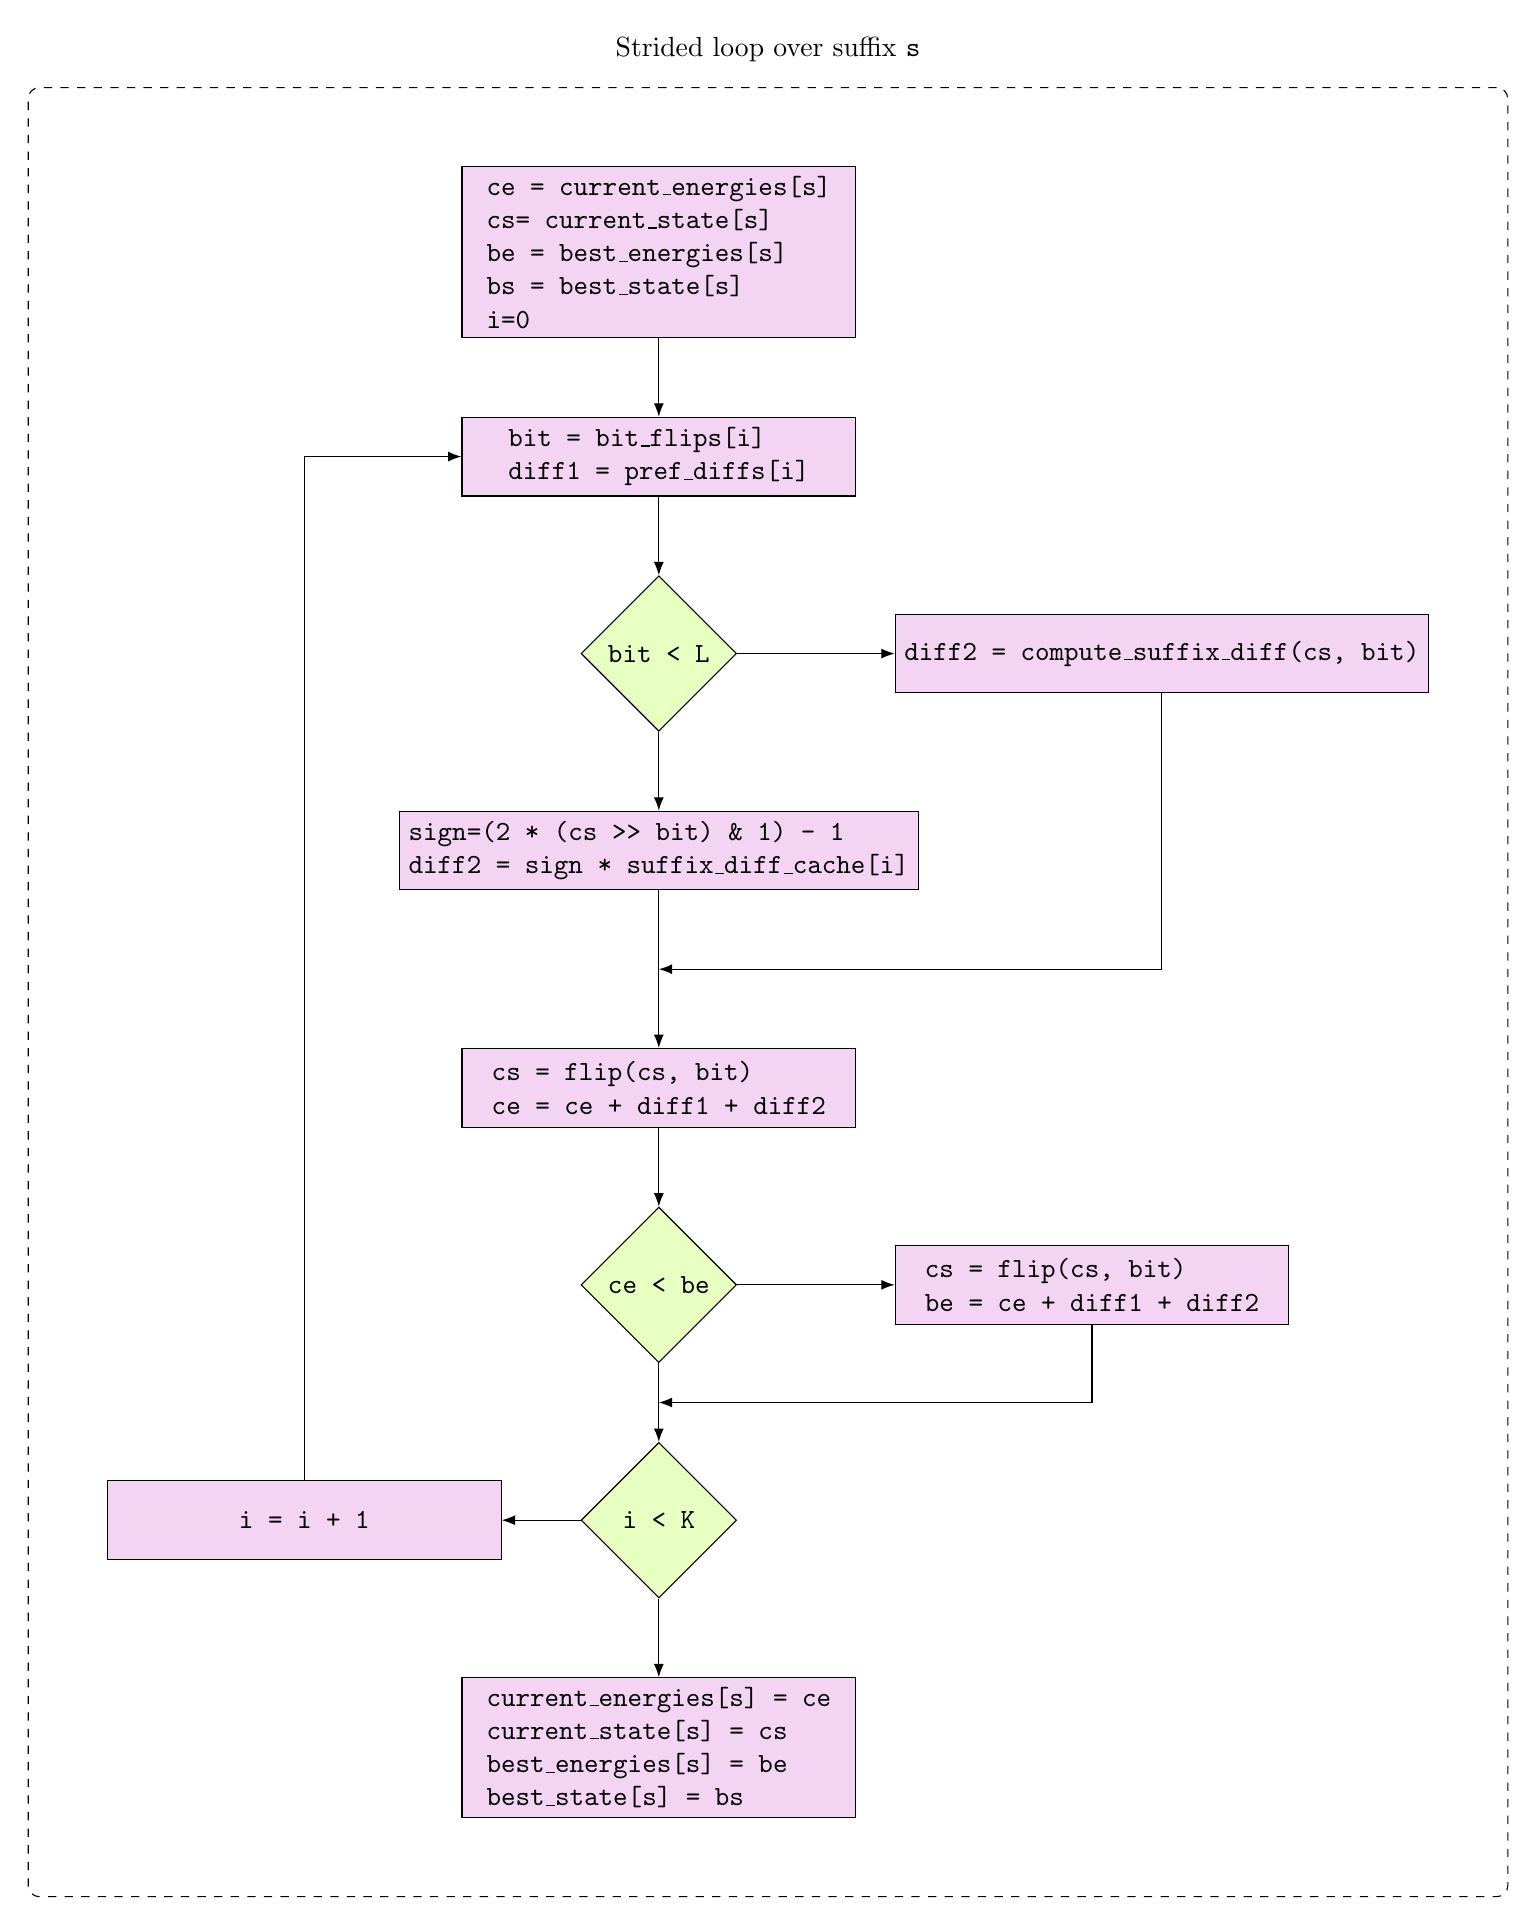
\begin{tikzpicture}[
memcell/.style={draw, rectangle, minimum width=0.2cm, minimum height=0.2cm},
    memarray/.style={minimum width=4cm, fill=white,minimum height=0.5cm, draw},
    energies/.style={memarray, nodes={memcell, fill=Energies}},
    rect/.style={minimum height=1cm, minimum width=5cm, fill=Rect, draw, rectangle, align=left},
    decision/.style={draw, align=center, diamond, fill=Decision},
    every node/.style={font={\normalsize}},
    brace/.style={decorate,decoration={brace,amplitude=5pt,mirror,raise=1mm}},
    brace2/.style={decorate,decoration={brace,amplitude=5pt,mirror,raise=4mm}},
    subroutine/.style={draw, rounded corners},
    subsubroutine/.style={subroutine,dashed,thick},
    gpuio/.style={-Latex,dashed}
    ]

    \node [rect] (load) {
      \texttt{ce = current\_energies[s]}\\
      \texttt{cs= current\_state[s]}\\
      \texttt{be = best\_energies[s]}\\
      \texttt{bs = best\_state[s]}\\
      \texttt{i=0}
    };
    \node [rect, below=1cm of load] (loop1) {\texttt{bit = bit\_flips[i]}\\\texttt{diff1 = pref\_diffs[i]}};
    \node [decision, below=1cm of loop1] (decision) {\texttt{bit < L}};
    \node [rect, right=2cm of decision] (diff2) {\texttt{diff2 = compute\_suffix\_diff(cs, bit)}};
    \node [rect, below=1cm of decision] (diff2alt) {
      \texttt{sign=(2 * (cs >> bit) \& 1) - 1}\\
      \texttt{diff2 = sign * suffix\_diff\_cache[i]}
    };
    \node [rect, below=2cm of diff2alt] (updatecurrent) {\texttt{cs = flip(cs, bit)}\\\texttt{ce = ce + diff1 + diff2}};
    \node [decision, below=1cm of updatecurrent] (decision2) {\texttt{ce < be}};
    \node [rect, right=2cm of decision2] (updatebest) {\texttt{cs = flip(cs, bit)}\\\texttt{be = ce + diff1 + diff2}};
    \node [decision, below=1cm of decision2] (decision3) {\texttt{~i < K~}};
    \node [rect, left=1cm of decision3] (increment) {\texttt{i = i + 1}};
    \node [rect, below=1cm of decision3] (update) {
      \texttt{current\_energies[s] = ce}\\
      \texttt{current\_state[s] = cs}\\
      \texttt{best\_energies[s] = be}\\
      \texttt{best\_state[s] = bs}
    };

    \node[
    fit=(update) (load) (diff2) (increment),
    draw,
    inner sep=1cm,
    rounded corners,
    dashed
    ] (stridedloop) {};

    \node[above=2mm of stridedloop] (label) {Strided loop over suffix \texttt{s}};
    \draw[-Latex] (load) -- (loop1);
    \draw[-Latex] (loop1) -- (decision);
    \draw[-Latex] (decision) -- (diff2);
    \draw[-Latex] (decision) -- (diff2alt);
    \draw[-Latex] (diff2alt) -- (updatecurrent);
    \draw[-Latex] (updatecurrent) -- (decision2);
    \draw[-Latex] (decision2) -- (updatebest);
    \draw[-Latex] (diff2) |- ($(diff2alt.south)!0.5!(updatecurrent.north)$);
    \draw[-Latex] (decision2) -- (decision3);
    \draw[-Latex] (decision3) -- (increment);
    \draw[-Latex] (increment) |- (loop1);
    \draw[-Latex] (decision3) -- (update);
    \draw[-Latex] (updatebest) |- ($(decision2)!0.5!(decision3)$);
\end{tikzpicture}
\end{document}
